\documentclass{beamer}

%
% Choose how your presentation looks.
%
% For more themes, color themes and font themes, see:
% http://deic.uab.es/~iblanes/beamer_gallery/index_by_theme.html
%
\mode<presentation>
{
  \usetheme{default}      % or try Darmstadt, Madrid, Warsaw, ...
  \usecolortheme{default} % or try albatross, beaver, crane, ...
  \usefonttheme{default}  % or try serif, structurebold, ...
  \setbeamertemplate{navigation symbols}{}
  \setbeamertemplate{caption}[numbered]
  \setbeamertemplate{footline}[page number]
  \setbeamercolor{frametitle}{fg=white}
  \setbeamercolor{footline}{fg=black}
} 

\usepackage[english]{babel}
\usepackage[utf8x]{inputenc}
\usepackage{tikz}
\usepackage{listings}
\usepackage{courier}

\xdefinecolor{darkblue}{rgb}{0.1,0.1,0.7}
\xdefinecolor{dianablue}{rgb}{0.18,0.24,0.31}
\definecolor{commentgreen}{rgb}{0,0.6,0}
\definecolor{stringmauve}{rgb}{0.58,0,0.82}

\lstset{ %
  backgroundcolor=\color{white},      % choose the background color
  basicstyle=\ttfamily\small,         % size of fonts used for the code
  breaklines=true,                    % automatic line breaking only at whitespace
  captionpos=b,                       % sets the caption-position to bottom
  commentstyle=\color{commentgreen},  % comment style
  escapeinside={\%*}{*)},             % if you want to add LaTeX within your code
  keywordstyle=\color{blue},          % keyword style
  stringstyle=\color{stringmauve},    % string literal style
  showstringspaces=false,
  showlines=true
}

\lstdefinelanguage{scala}{
  morekeywords={abstract,case,catch,class,def,%
    do,else,extends,false,final,finally,%
    for,if,implicit,import,match,mixin,%
    new,null,object,override,package,%
    private,protected,requires,return,sealed,%
    super,this,throw,trait,true,try,%
    type,val,var,while,with,yield},
  otherkeywords={=>,<-,<\%,<:,>:,\#,@},
  sensitive=true,
  morecomment=[l]{//},
  morecomment=[n]{/*}{*/},
  morestring=[b]",
  morestring=[b]',
  morestring=[b]"""
}

\title[2016-11-07-rootteam-root4j]{Reading ROOT data in Java and Spark}
\author{Jim Pivarski}
\institute{Princeton -- DIANA}
\date{November 7, 2016}

\begin{document}

\logo{\pgfputat{\pgfxy(0.11, 8)}{\pgfbox[right,base]{\tikz{\filldraw[fill=dianablue, draw=none] (0 cm, 0 cm) rectangle (50 cm, 1 cm);}}}\pgfputat{\pgfxy(0.11, -0.6)}{\pgfbox[right,base]{\tikz{\filldraw[fill=dianablue, draw=none] (0 cm, 0 cm) rectangle (50 cm, 1 cm);}
\includegraphics[height=0.99 cm]{diana-hep-logo.png}\tikz{\filldraw[fill=dianablue, draw=none] (0 cm, 0 cm) rectangle (4.9 cm, 1 cm);}}}}

\begin{frame}
  \titlepage
\end{frame}

\logo{\pgfputat{\pgfxy(0.11, 8)}{\pgfbox[right,base]{\tikz{\filldraw[fill=dianablue, draw=none] (0 cm, 0 cm) rectangle (50 cm, 1 cm);}
\includegraphics[height=1 cm]{diana-hep-logo.png}}}}

% Uncomment these lines for an automatically generated outline.
%\begin{frame}{Outline}
%  \tableofcontents
%\end{frame}

\begin{frame}{Motivation}
\vspace{0.25 cm}
In a physics analysis using Spark {\small (Oliver Gutsche, Matteo Cremonesi, Cristina Mantilla)}, the first step is data access.

\vspace{0.25 cm}
Hard to cross the boundary between ROOT's C++ runtime and Spark's Java Virtual Machine (JVM).

\vspace{0.25 cm}
\begin{uncoverenv}<2->
\textcolor{darkblue}{Four methods considered:}
\begin{enumerate}
\item Convert all data from ROOT to another format (Avro).
\item Access ROOT inside the JVM via JNI.
\item Access ROOT as an external process (pipe or socket).
\item Run PyROOT in PySpark.
\end{enumerate}
\end{uncoverenv}

\vspace{0.25 cm}
\begin{uncoverenv}<3->
The 2016 analysis used option \textcolor{darkblue}{\#1}, but it's not ideal.
\begin{itemize}
\item Separate conversion step before running Spark.
\item Two copies of the data: extra version control and disk usage.
\end{itemize}
\end{uncoverenv}
\end{frame}

\begin{frame}{Previously rejected solution}
\vspace{0.25 cm}
\begin{center}
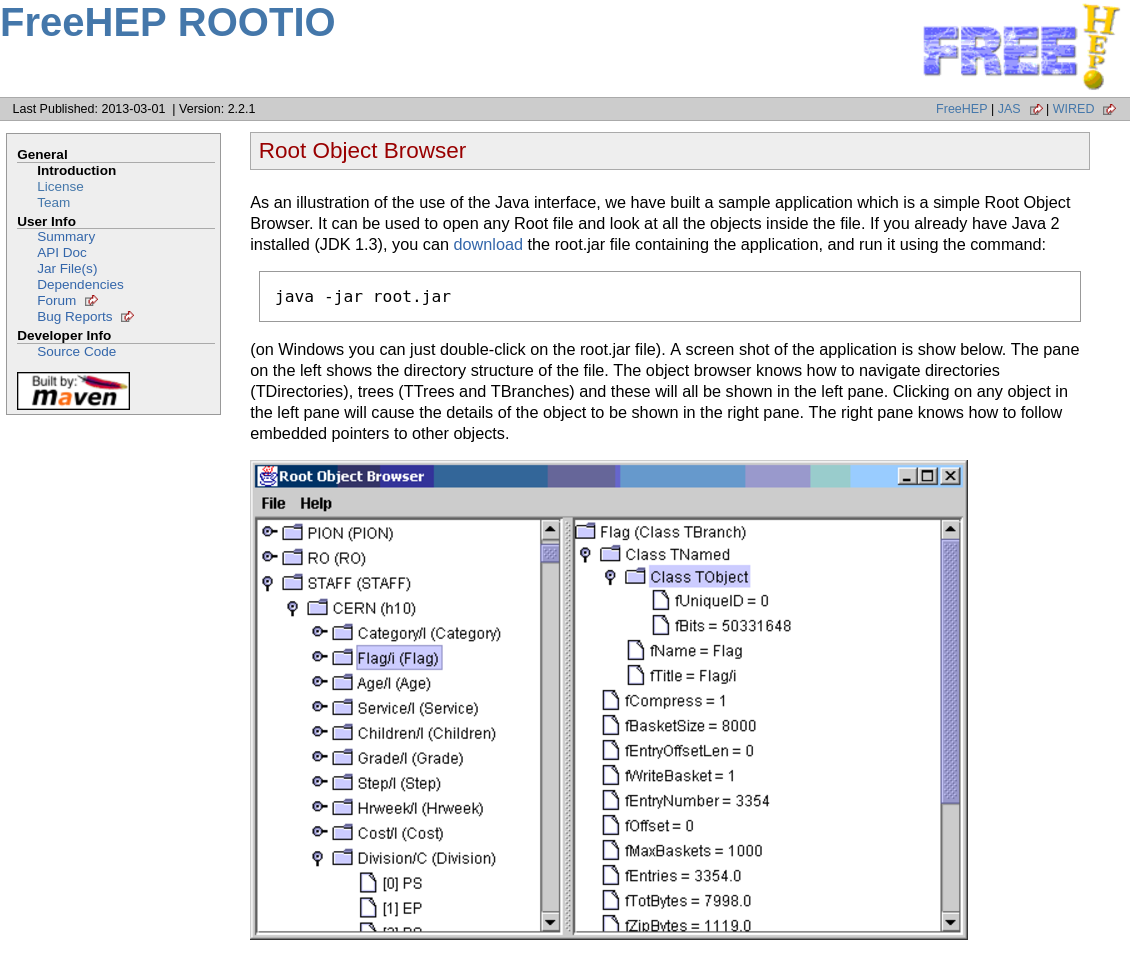
\includegraphics[width=0.9\linewidth]{rootio-screenshot.png}
\end{center}
\end{frame}

\begin{frame}{Previously rejected solution}
\vspace{0.35 cm}
\begin{block}{FreeHEP ROOTIO \scriptsize (\textcolor{blue}{\url{http://java.freehep.org/freehep-rootio/}})}
\vspace{-0.1 cm}
\begin{itemize}
\item Re-implementation of ROOT's I/O in Java.
\item Used as a backend in Java Analysis Studio (JAS).
\item First talks by Tony Johnson in 2001, commits trail off $\sim$2010.
\end{itemize}
\end{block}

\vspace{-0.25 cm}
\begin{uncoverenv}<2->
\begin{block}{Why not?}
\vspace{-0.1 cm}
\begin{itemize}
\item Lack of documentation; high-level interface described on website no longer exists.
\item Immediately failed when presented with recent ROOT file.
\item Can't get in touch with Tony Johnson.
\end{itemize}
\end{block}
\end{uncoverenv}

\vspace{-0.25 cm}
\begin{uncoverenv}<3->
\begin{block}{Why now?}
\vspace{-0.1 cm}
\begin{itemize}
\item I reexamined its low-level interface (direct access to TBranches/TBaskets), and it works!
\item Only 3 minor bug-fixes needed to read complex CMS AOD.
\end{itemize}
\end{block}
\end{uncoverenv}
\end{frame}

\begin{frame}{}
\begin{block}{Advantages of a pure-Java reader}
\begin{itemize}
\item No intermediate files: can copy ROOT files directly into HDFS and use them.
\item 


\end{itemize}
\end{block}
\end{frame}



\end{document}
